% Options for packages loaded elsewhere
\PassOptionsToPackage{unicode}{hyperref}
\PassOptionsToPackage{hyphens}{url}
\PassOptionsToPackage{dvipsnames,svgnames,x11names}{xcolor}
%
\documentclass[
  letterpaper,
  DIV=11,
  numbers=noendperiod]{scrreprt}

\usepackage{amsmath,amssymb}
\usepackage{iftex}
\ifPDFTeX
  \usepackage[T1]{fontenc}
  \usepackage[utf8]{inputenc}
  \usepackage{textcomp} % provide euro and other symbols
\else % if luatex or xetex
  \usepackage{unicode-math}
  \defaultfontfeatures{Scale=MatchLowercase}
  \defaultfontfeatures[\rmfamily]{Ligatures=TeX,Scale=1}
\fi
\usepackage{lmodern}
\ifPDFTeX\else  
    % xetex/luatex font selection
\fi
% Use upquote if available, for straight quotes in verbatim environments
\IfFileExists{upquote.sty}{\usepackage{upquote}}{}
\IfFileExists{microtype.sty}{% use microtype if available
  \usepackage[]{microtype}
  \UseMicrotypeSet[protrusion]{basicmath} % disable protrusion for tt fonts
}{}
\makeatletter
\@ifundefined{KOMAClassName}{% if non-KOMA class
  \IfFileExists{parskip.sty}{%
    \usepackage{parskip}
  }{% else
    \setlength{\parindent}{0pt}
    \setlength{\parskip}{6pt plus 2pt minus 1pt}}
}{% if KOMA class
  \KOMAoptions{parskip=half}}
\makeatother
\usepackage{xcolor}
\setlength{\emergencystretch}{3em} % prevent overfull lines
\setcounter{secnumdepth}{5}
% Make \paragraph and \subparagraph free-standing
\ifx\paragraph\undefined\else
  \let\oldparagraph\paragraph
  \renewcommand{\paragraph}[1]{\oldparagraph{#1}\mbox{}}
\fi
\ifx\subparagraph\undefined\else
  \let\oldsubparagraph\subparagraph
  \renewcommand{\subparagraph}[1]{\oldsubparagraph{#1}\mbox{}}
\fi


\providecommand{\tightlist}{%
  \setlength{\itemsep}{0pt}\setlength{\parskip}{0pt}}\usepackage{longtable,booktabs,array}
\usepackage{calc} % for calculating minipage widths
% Correct order of tables after \paragraph or \subparagraph
\usepackage{etoolbox}
\makeatletter
\patchcmd\longtable{\par}{\if@noskipsec\mbox{}\fi\par}{}{}
\makeatother
% Allow footnotes in longtable head/foot
\IfFileExists{footnotehyper.sty}{\usepackage{footnotehyper}}{\usepackage{footnote}}
\makesavenoteenv{longtable}
\usepackage{graphicx}
\makeatletter
\def\maxwidth{\ifdim\Gin@nat@width>\linewidth\linewidth\else\Gin@nat@width\fi}
\def\maxheight{\ifdim\Gin@nat@height>\textheight\textheight\else\Gin@nat@height\fi}
\makeatother
% Scale images if necessary, so that they will not overflow the page
% margins by default, and it is still possible to overwrite the defaults
% using explicit options in \includegraphics[width, height, ...]{}
\setkeys{Gin}{width=\maxwidth,height=\maxheight,keepaspectratio}
% Set default figure placement to htbp
\makeatletter
\def\fps@figure{htbp}
\makeatother

\KOMAoption{captions}{tableheading}
\makeatletter
\makeatother
\makeatletter
\@ifpackageloaded{bookmark}{}{\usepackage{bookmark}}
\makeatother
\makeatletter
\@ifpackageloaded{caption}{}{\usepackage{caption}}
\AtBeginDocument{%
\ifdefined\contentsname
  \renewcommand*\contentsname{Table of contents}
\else
  \newcommand\contentsname{Table of contents}
\fi
\ifdefined\listfigurename
  \renewcommand*\listfigurename{List of Figures}
\else
  \newcommand\listfigurename{List of Figures}
\fi
\ifdefined\listtablename
  \renewcommand*\listtablename{List of Tables}
\else
  \newcommand\listtablename{List of Tables}
\fi
\ifdefined\figurename
  \renewcommand*\figurename{Figure}
\else
  \newcommand\figurename{Figure}
\fi
\ifdefined\tablename
  \renewcommand*\tablename{Table}
\else
  \newcommand\tablename{Table}
\fi
}
\@ifpackageloaded{float}{}{\usepackage{float}}
\floatstyle{ruled}
\@ifundefined{c@chapter}{\newfloat{codelisting}{h}{lop}}{\newfloat{codelisting}{h}{lop}[chapter]}
\floatname{codelisting}{Listing}
\newcommand*\listoflistings{\listof{codelisting}{List of Listings}}
\makeatother
\makeatletter
\@ifpackageloaded{caption}{}{\usepackage{caption}}
\@ifpackageloaded{subcaption}{}{\usepackage{subcaption}}
\makeatother
\makeatletter
\@ifpackageloaded{tcolorbox}{}{\usepackage[skins,breakable]{tcolorbox}}
\makeatother
\makeatletter
\@ifundefined{shadecolor}{\definecolor{shadecolor}{rgb}{.97, .97, .97}}
\makeatother
\makeatletter
\makeatother
\makeatletter
\makeatother
\ifLuaTeX
  \usepackage{selnolig}  % disable illegal ligatures
\fi
\IfFileExists{bookmark.sty}{\usepackage{bookmark}}{\usepackage{hyperref}}
\IfFileExists{xurl.sty}{\usepackage{xurl}}{} % add URL line breaks if available
\urlstyle{same} % disable monospaced font for URLs
\hypersetup{
  pdftitle={Introduction},
  pdfauthor={Nooriza Maharani},
  colorlinks=true,
  linkcolor={blue},
  filecolor={Maroon},
  citecolor={Blue},
  urlcolor={Blue},
  pdfcreator={LaTeX via pandoc}}

\title{Introduction}
\author{Nooriza Maharani}
\date{January 21, 2025}

\begin{document}
\maketitle
\ifdefined\Shaded\renewenvironment{Shaded}{\begin{tcolorbox}[boxrule=0pt, interior hidden, enhanced, sharp corners, breakable, frame hidden, borderline west={3pt}{0pt}{shadecolor}]}{\end{tcolorbox}}\fi

\renewcommand*\contentsname{Table of contents}
{
\hypersetup{linkcolor=}
\setcounter{tocdepth}{2}
\tableofcontents
}
\bookmarksetup{startatroot}

\hypertarget{rs-learning-diary}{%
\chapter{RS Learning Diary}\label{rs-learning-diary}}

This is a Quarto book to document my learning journey in \textbf{Remote
Sensing Cities and Environments} course during my time at CASA UCL
24/25, offering insights learned, its applications, and my own
reflections. The module is based on Dr Andrew Maclachlan github page
{[}\href{https://andrewmaclachlan.github.io/CASA0023/.}{here}{]}.

*For those of you who also want to learn Geographic Information Scicene
beyond `typical GIS' Software, as in use R-Studio, you could also visit
his other github page
{[}\href{https://andrewmaclachlan.github.io/CASA0005repo/index.html}{here}{]}.

\begin{center}\rule{0.5\linewidth}{0.5pt}\end{center}

\hypertarget{introduction}{%
\section{Introduction}\label{introduction}}

Hi, I'm Nooriza, a student currently pursuing a Master's degree in Urban
Spatial Science at UCL. I have an academic background in Geography with
a specialization in Regional Development Studies and have several
substantial work experience in government consultancies in Indonesia.

\hypertarget{why-do-i-choose-this-module}{%
\section{Why do I choose this
module?}\label{why-do-i-choose-this-module}}

The reason I take Remote Sensing course is my desire to know \emph{how
it feels to be a bird, seeing things from above, and to see the unseen.}
Don't we agree that remote sensing offers perspectives far beyond what
our human eyes can naturally perceive?

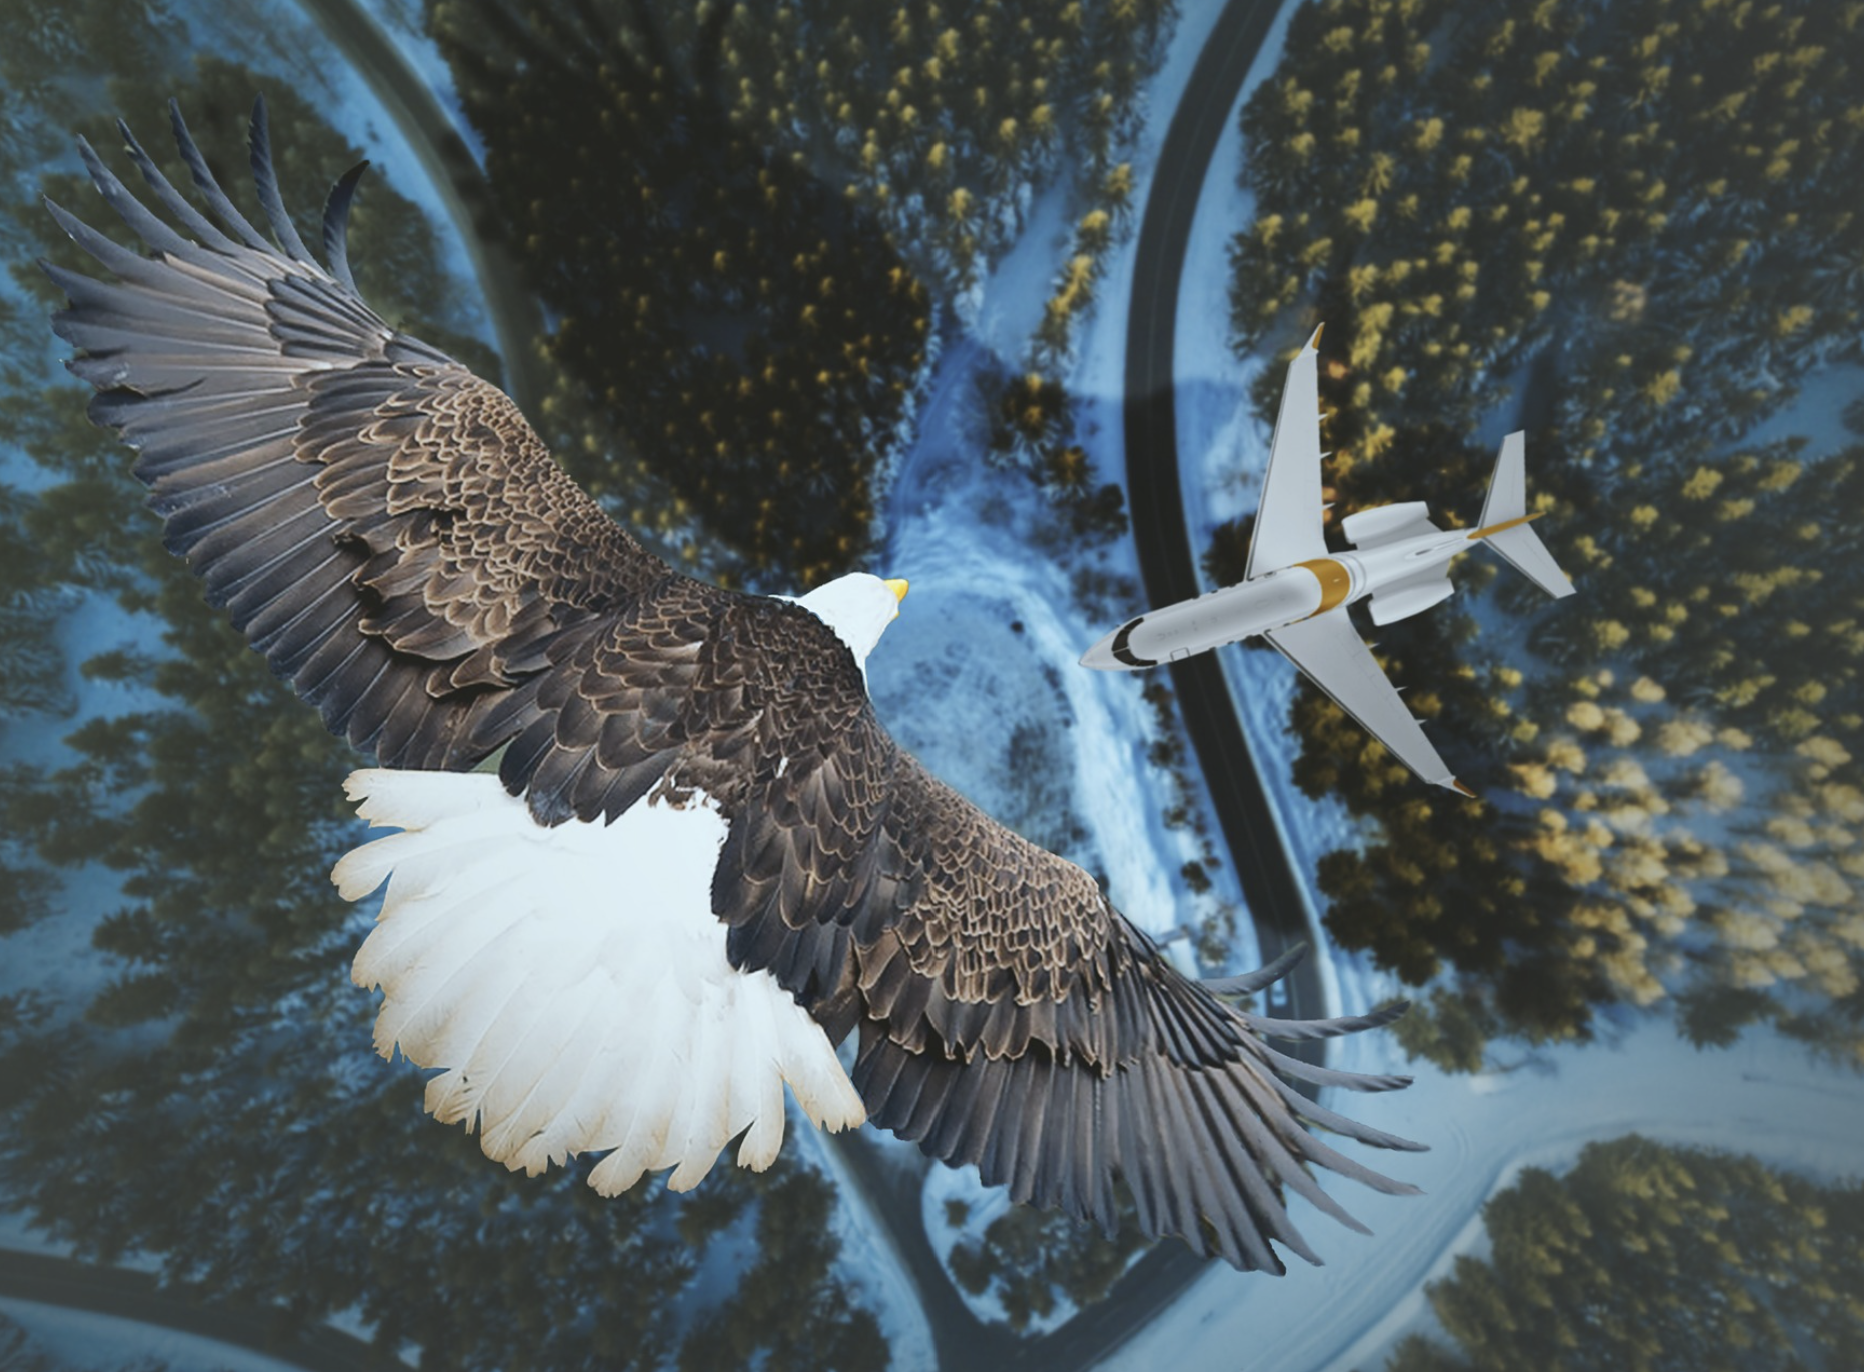
\includegraphics[width=5.07292in,height=\textheight]{images/clipboard-2217286199.png}

source :
\href{https://chirpforbirds.com/nature-advocacy/biomimicry-and-birds/}{Biomimicry
and Birds}

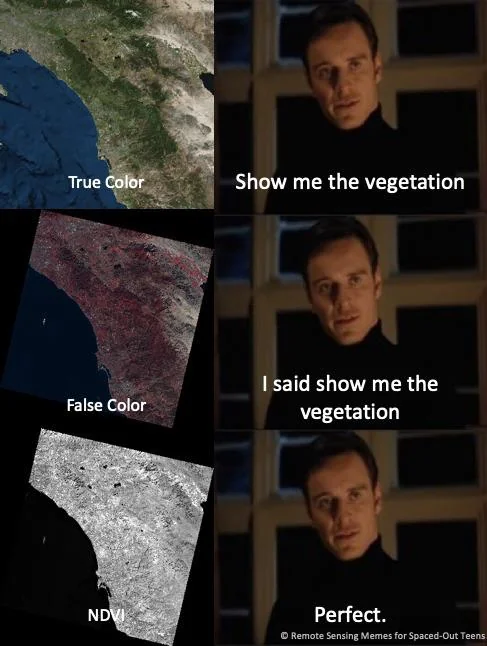
\includegraphics{images/ggd7oxp59qb31.jpeg}

(c) Remote Sensing Memes for Spaced-Out Teens

Meanwhile, practically, learning this course will, hopefully, help me
address the challenges I faced during my previous work in Indonesia. For
example, while working on a project focused on healthcare accessibility
across hundreds of small islands, we struggled to obtain real-time data
to identify which islands were inhabited and which were not.
Additionally, we faced challenges in determining which islands had ports
suitable for docking ships. I believe that applying remote sensing data
is both cost- and time-efficient in helping the government maintain more
precise and up-to-date data, which is particularly important in world's
largest archipelago country like Indonesia.

Feel free to explore my site to learn more about my learning experience.
Hope it helps!

\bookmarksetup{startatroot}

\hypertarget{week-1}{%
\chapter{Week 1}\label{week-1}}

\bookmarksetup{startatroot}

\hypertarget{week-1-getting-to-know-remote-sensing}{%
\chapter{Week 1 : Getting to Know Remote
Sensing}\label{week-1-getting-to-know-remote-sensing}}

\begin{itemize}
\tightlist
\item
  \textbf{Sneak Peak}
\end{itemize}

This week is an introduction of Remote Sensing courses, introducing 2
sources of imagery :

\begin{enumerate}
\def\labelenumi{\arabic{enumi}.}
\item
  Landsat-8

  The Landsat 8 satellite has a 16-day revisit cycle, meaning it can
  capture imagery of the same location every 16 day. This period would
  be advantageous to monitor changes at moderate pace, as its revisit
  time is every 16 days.
\end{enumerate}

\begin{itemize}
\item
  \begin{figure}

  {\centering 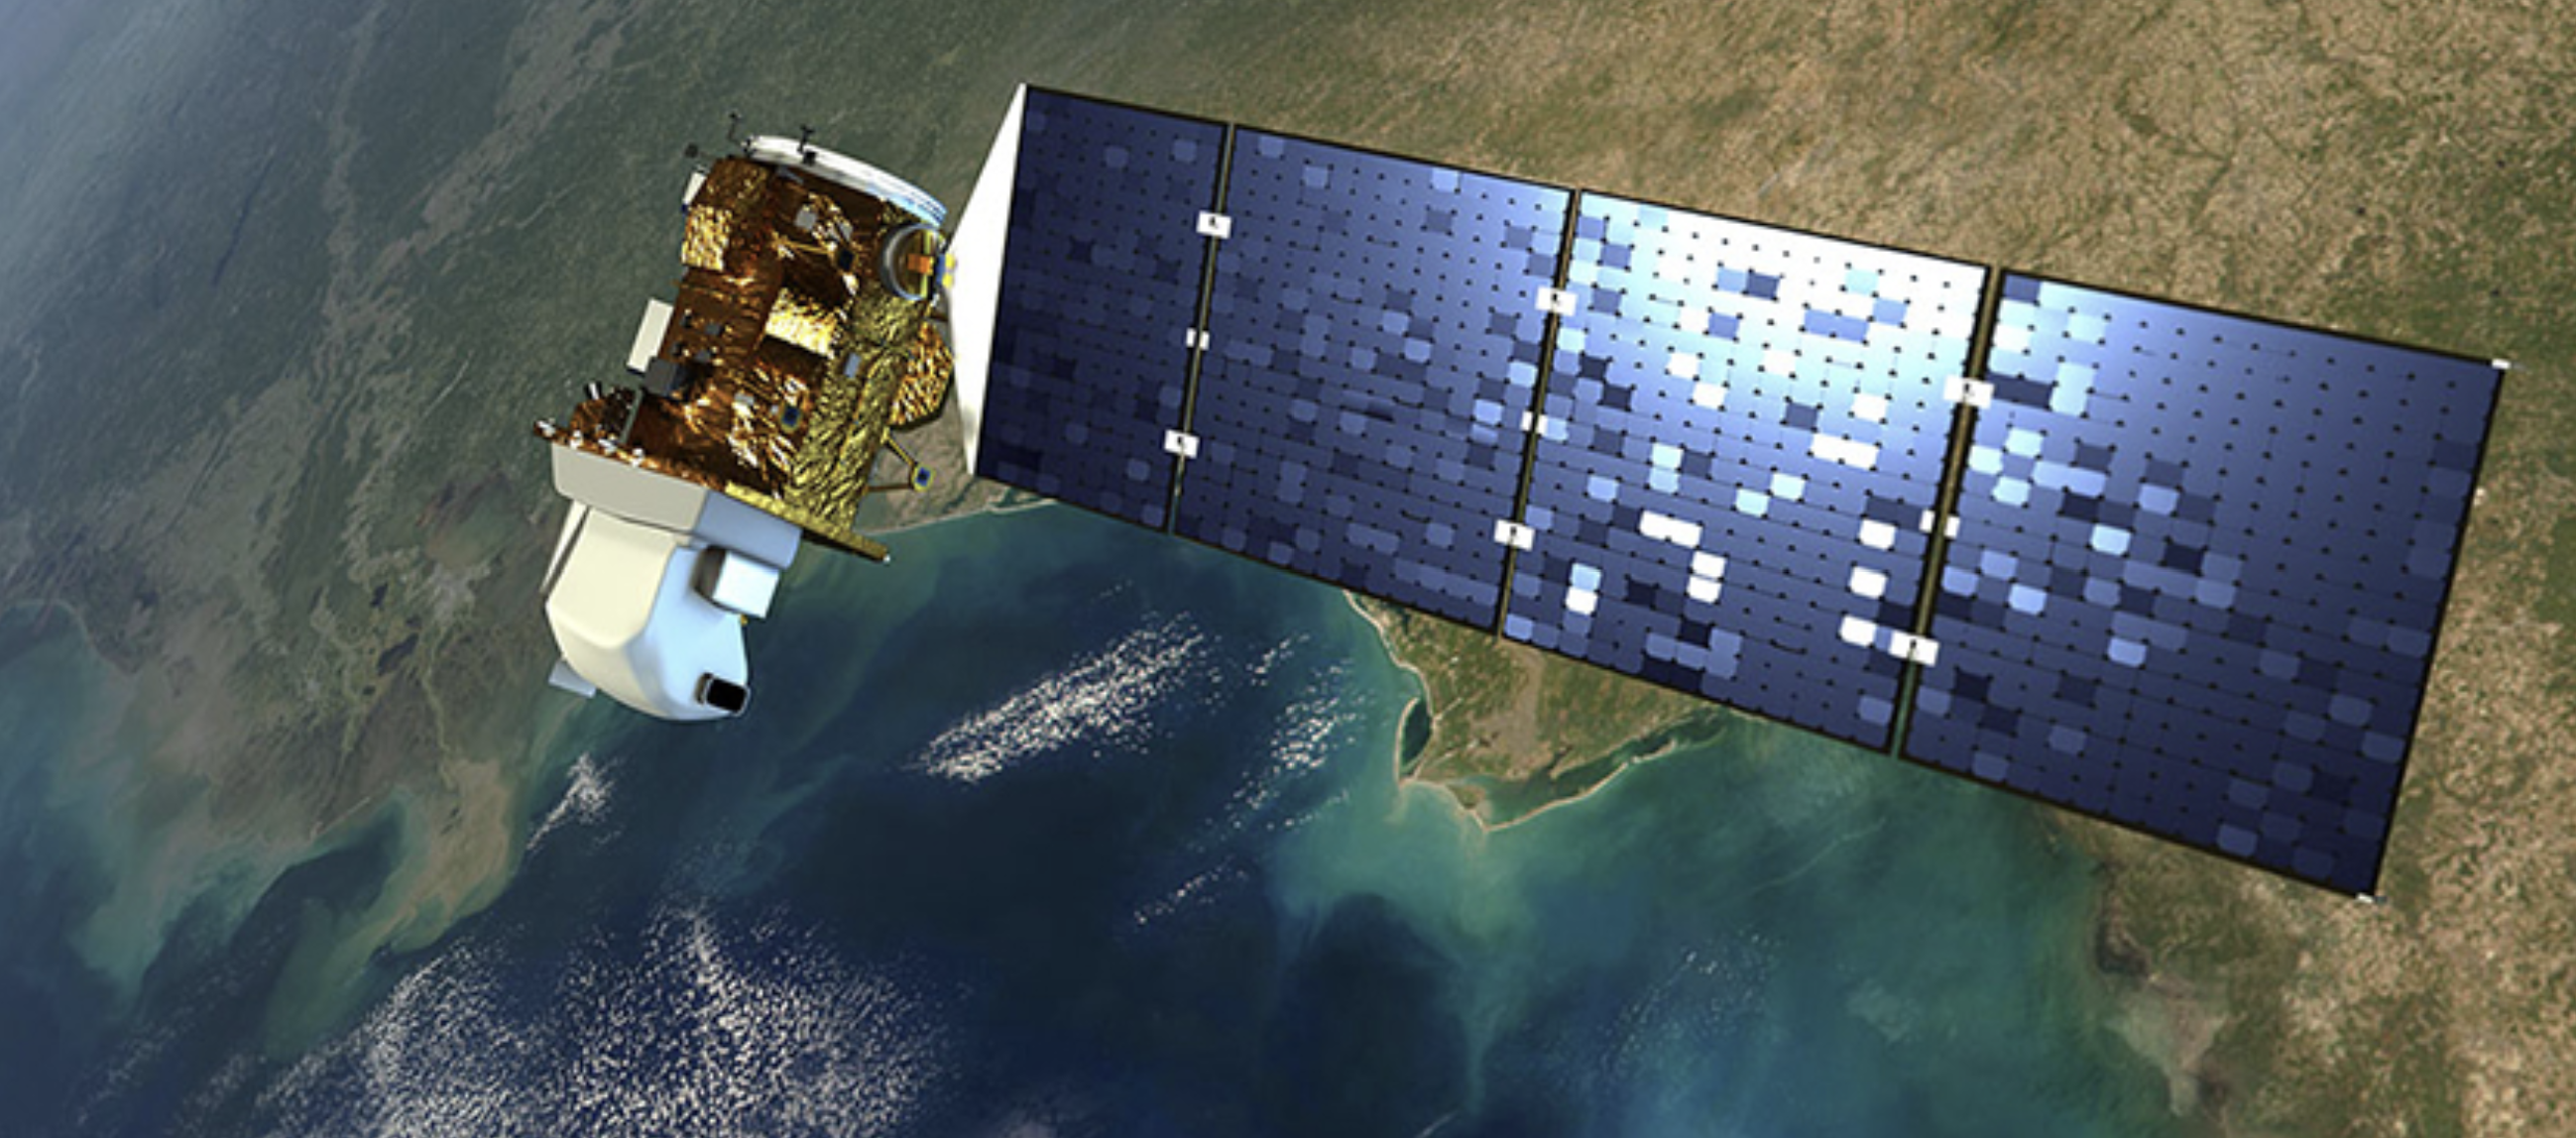
\includegraphics[width=4.1875in,height=\textheight]{images/clipboard-1188776161.png}

  }

  \caption{Copyright © NASA}

  \end{figure}
\end{itemize}

\begin{enumerate}
\def\labelenumi{\arabic{enumi}.}
\setcounter{enumi}{1}
\item
  Sentinel 2A

  Sentinel 2 revisits the earth every 5 days (using both satellite A and
  B), meaning that it provides frequent observations and make it
  suitable to monitor rapid changes.
\end{enumerate}

\begin{itemize}
\item
  \begin{figure}

  {\centering 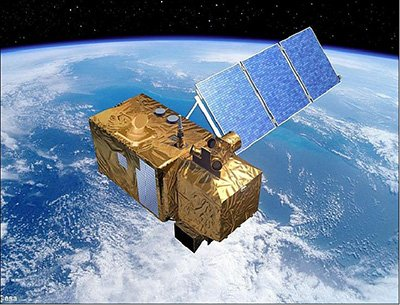
\includegraphics{images/clipboard-3938270325.png}

  }

  \caption{Copyright © ESA and AIRBUS Defence \& Space.}

  \end{figure}

  Each has their own characteristics, while Sentinel-2A has 10m spatial
  resolution Landsat-8 has 30m resolution. If we want to compare its
  spectral resolution we have to either upgrade or downgrade, usually
  downgrading the higher spatial resolution of Sentinel-2 (10m) to match
  Landsat's (30m) is the preferred approach.
\end{itemize}

\bookmarksetup{startatroot}

\hypertarget{application}{%
\chapter{Application}\label{application}}

\textbf{In what ways can we use Sentinel and Landsat data?}

\begin{itemize}
\item
  Sentinel-2 (operated by ESA) has \emph{13 spectral bands} across a
  wide range of wavelengths, which are especially useful for vegetation
  monitoring, land cover classification, and agricultural applications.
\item
  Landsat 8 (operated by NASA and USGS) has \emph{11 spectral bands},
  which cover a similar range of wavelengths to Sentinel-2 but with
  fewer bands. Landsat 8 provides excellent coverage for land monitoring
  and vegetation studies as well.
\end{itemize}

\textbf{They both could be used to vegetation monitoring,
well\ldots\ldots..are they really that difference?}

\begin{itemize}
\item
  Sentinel-2 has more bands overall, with additional Red Edge bands, a
  higher spatial resolution (10m for key bands), and a Water Vapor band.
  This makes it more suited for \textbf{\emph{detailed vegetation
  analysis}}, agricultural monitoring, and atmospheric studies. In the
  paper\ldots..
\item
  Landsat 8, while having fewer bands, provides excellent coverage with
  a broader range of SWIR bands, and the addition of two thermal
  infrared bands makes it strong for land surface temperature and other
  \emph{\textbf{thermal analyses}.}
\end{itemize}

\bookmarksetup{startatroot}

\hypertarget{week-2}{%
\chapter{Week 2}\label{week-2}}

\bookmarksetup{startatroot}

\hypertarget{xaringan}{%
\chapter{Xaringan}\label{xaringan}}

Lecture this week reminded me of one of powerful figure in Uchiha Clan,
the one who can manipulate reality once he activates this-so-called
Xaringan. Well, but this Xaringan is not related to figures in Konoha's
world but related to a certain library in R Studio that enable us to
create neat HTML slides in R.

\bookmarksetup{startatroot}

\hypertarget{hows-xaringan-look-like}{%
\chapter{How's xaringan look like?}\label{hows-xaringan-look-like}}

\bookmarksetup{startatroot}

\hypertarget{week-3}{%
\chapter{Week 3}\label{week-3}}

\bookmarksetup{startatroot}

\hypertarget{week-4}{%
\chapter{Week 4}\label{week-4}}



\end{document}
